\chapter*{Setting up your robot using tf:}

\begin{verbatim}
http://www.ros.org/wiki/navigation/Tutorials/RobotSetup/TF


Setting up your robot using tf
Description: This tutorial provides a guide to set up your robot to start using tf.

Tutorial Level: BEGINNER

Next Tutorial: Learn how to have the robot state publisher do all the tf publishing for you: using the robot state publisher on your own robot

Tabla de Contenidos

   1. Transform Configuration
   2. Writing Code
   3. Broadcasting a Transform
   4. Using a Transform
   5. Building the Code
   6. Running the Code

Transform Configuration

Many ros packages require the transform tree of a robot to be published using the tf software library. At an abstract level, a transform tree defines offsets in terms of both translation and rotation between different coordinate frames. To make this more concrete, consider the example of a simple robot that has a mobile base with a single laser mounted on top of it. In referring to the robot let's define two coordinate frames: one corresponding to the center point of the base of the robot and one for the center point of the laser that is mounted on top of the base. Let's also give them names for easy reference. We'll call the coordinate frame attached to the mobile base "base_link" and we'll call the coordinate frame attached to the laser "base_laser."

At this point, let's assume that we have some data from the laser in the form of distances from the laser's center point. In other words, we have some data in the "base_laser" coordinate frame. Now suppose we want to take this data and use it to help the mobile base avoid obstacles in the world. To do this successfully, we need a way of transforming the laser scan we've received from the "base_laser" frame to the "base_link" frame. In essence, we need to define a relationship between the "base_laser" and "base_link" coordinate frames.

simple_robot.png

In defining this relationship, assume we know that the laser is mounted 10cm forward and 20cm above the center point of the mobile base. This gives us a translational offset that relates the "base_link" frame to the "base_laser" frame. Specifically, we know that to get data from the "base_link" frame to the "base_laser" frame we must apply a translation of (x: 0.1m, y: 0.0m, z: 0.2m), and to get data from the "base_laser" frame to the "base_link" frame we must apply the opposite translation (x: -0.1m, y: 0.0m, z: -0.20m).

We could choose to manage this relationship ourselves, meaning storing and applying the appropriate translations between the frames when necessary, but this becomes a real pain as the number of coordinate frames increase. Luckily, however, we don't have to do this work ourselves. Instead we'll define the relationship between "base_link" and "base_laser" once using tf and let it manage the transformation between the two coordinate frames for us.

To define and store the relationship between the "base_link" and "base_laser" frames using tf, we need to add them to a transform tree. Conceptually, each node in the transform tree corresponds to a coordinate frame and each edge corresponds to the transform that needs to be applied to move from the current node to its child. Tf uses a tree structure to guarantee that there is only a single traversal that links any two coordinate frames together, and assumes that all edges in the tree are directed from parent to child nodes.

tf_robot.png

To create a transform tree for our simple example, we'll create two nodes, one for the "base_link" coordinate frame and one for the "base_laser" coordinate frame. To create the edge between them, we first need to decide which node will be the parent and which will be the child. Remember, this distinction is important because tf assumes that all transforms move from parent to child. Let's choose the "base_link" coordinate frame as the parent because as other pieces/sensors are added to the robot, it will make the most sense for them to relate to the "base_laser" frame by traversing through the "base_link" frame. This means the transform associated with the edge connecting "base_link" and "base_laser" should be (x: 0.1m, y: 0.0m, z: 0.2m). With this transform tree set up, converting the laser scan received in the "base_laser" frame to the "base_link" frame is as simple as making a call to the tf library. Our robot can use this information to reason about laser scans in the "base_link" frame and safely plan around obstacles in its environment.

Writing Code

Hopefully, the above example helped to understand tf on a conceptual level. Now, we've got to take the transform tree and create it with code. For this example, familiarity with ROS is assumed, so make sure to check out the ROS Documentation if any terms or concepts are unfamiliar.

Suppose that we have the high level task described above of taking points in the "base_laser" frame and transforming them to the "base_link" frame. The first thing we need to do is to create a node that will be responsible for publishing the transforms in our system. Next, we'll have to create a node to listen to the transform data published over ROS and apply it to transform a point. We'll start by creating a package for the source code to live in and we'll give it a simple name like "robot_setup_tf" We'll have dependencies on roscpp, tf, and geometry_msgs.

roscreate-pkg robot_setup_tf roscpp tf geometry_msgs

Broadcasting a Transform

Now that we've got our package, we need to create the node that will do the work of broadcasting the base_laser → base_link transform over ROS. In the robot_setup_tf package you just created, fire up your favorite editor and paste the following code into the src/tf_broadcaster.cpp file.

[des]activar nros. de línea

   1 #include <ros/ros.h>
   2 #include <tf/transform_broadcaster.h>
   3 
   4 int main(int argc, char** argv){
   5   ros::init(argc, argv, "robot_tf_publisher");
   6   ros::NodeHandle n;
   7 
   8   ros::Rate r(100);
   9 
  10   tf::TransformBroadcaster broadcaster;
  11 
  12   while(n.ok()){
  13     broadcaster.sendTransform(
  14       tf::StampedTransform(
  15         tf::Transform(tf::Quaternion(0, 0, 0, 1), tf::Vector3(0.1, 0.0, 0.2)),
  16         ros::Time::now(),"base_link", "base_laser"));
  17     r.sleep();
  18   }
  19 }

Now, let's take a look at the code that is relevant to publishing the base_link → base_laser transform in more detail.

[des]activar nros. de línea

   2 #include <tf/transform_broadcaster.h>

The tf package provides an implementation of a tf::TransformBroadcaster to help make the task of publishing transforms easier. To use the TransformBroadcaster, we need to include the tf/transform_broadcaster.h header file.

[des]activar nros. de línea

  10   tf::TransformBroadcaster broadcaster;

Here, we create a TransformBroadcaster object that we'll use later to send the base_link → base_laser` transform over the wire.

[des]activar nros. de línea

  13     broadcaster.sendTransform(
  14       tf::StampedTransform(
  15         tf::Transform(tf::Quaternion(0, 0, 0, 1), tf::Vector3(0.1, 0.0, 0.2)),
  16         ros::Time::now(),"base_link", "base_laser"));

This is where the real work is done. Sending a transform with a TransformBroadcaster requires five arguments. First, we pass in the rotation transform, which is specified by a btQuaternion for any rotation that needs to occur between the two coordinate frames. In this case, we want no apply no rotation, so we send in a btQuaternion constructed from pitch, roll, and yaw values equal to zero. Second, a btVector3 for any translation that we'd like to apply. We do, however, want to apply a translation, so we create a btVector3 corresponding to the laser's x offset of 10cm and z offset of 20cm from the robot base. Third, we need to give the transform being published a timestamp, we'll just stamp it with ros::Time::now(). Fourth, we need to pass the name of the parent node of the link we're creating, in this case "base_link." Fifth, we need to pass the name of the child node of the link we're creating, in this case "base_laser."

Using a Transform

Above, we created a node that publishes the base_laser → base_link transform over ROS. Now, we're going to write a node that will use that transform to take a point in the "base_laser" frame and transform it to a point in the "base_link" frame. Once again, we'll start by pasting the code below into a file and follow up with a more detailed explanation. In the robot_setup_tf package, create a file called src/tf_listener.cpp and paste the following:

[des]activar nros. de línea

   1 #include <ros/ros.h>
   2 #include <geometry_msgs/PointStamped.h>
   3 #include <tf/transform_listener.h>
   4 
   5 void transformPoint(const tf::TransformListener& listener){
   6   //we'll create a point in the base_laser frame that we'd like to transform to the base_link frame
   7   geometry_msgs::PointStamped laser_point;
   8   laser_point.header.frame_id = "base_laser";
   9 
  10   //we'll just use the most recent transform available for our simple example
  11   laser_point.header.stamp = ros::Time();
  12 
  13   //just an arbitrary point in space
  14   laser_point.point.x = 1.0;
  15   laser_point.point.y = 0.2;
  16   laser_point.point.z = 0.0;
  17 
  18   try{
  19     geometry_msgs::PointStamped base_point;
  20     listener.transformPoint("base_link", laser_point, base_point);
  21 
  22     ROS_INFO("base_laser: (%.2f, %.2f. %.2f) -----> base_link: (%.2f, %.2f, %.2f) at time %.2f",
  23         laser_point.point.x, laser_point.point.y, laser_point.point.z,
  24         base_point.point.x, base_point.point.y, base_point.point.z, base_point.header.stamp.toSec());
  25   }
  26   catch(tf::TransformException& ex){
  27     ROS_ERROR("Received an exception trying to transform a point from \"base_laser\" to \"base_link\": %s", ex.what());
  28   }
  29 }
  30 
  31 int main(int argc, char** argv){
  32   ros::init(argc, argv, "robot_tf_listener");
  33   ros::NodeHandle n;
  34 
  35   tf::TransformListener listener(ros::Duration(10));
  36 
  37   //we'll transform a point once every second
  38   ros::Timer timer = n.createTimer(ros::Duration(1.0), boost::bind(&transformPoint, boost::ref(listener)));
  39 
  40   ros::spin();
  41 
  42 }

Ok... now we'll walk through the important bits step by step.

[des]activar nros. de línea

   3 #include <tf/transform_listener.h>

Here, we include the tf/transform_listener.h header file that we'll need to create a tf::TransformListener. A TransformListener object automatically subscribes to the transform message topic over ROS and manages all transform data coming in over the wire.

[des]activar nros. de línea

   5 void transformPoint(const tf::TransformListener& listener){

We'll create a function that, given a TransformListener, takes a point in the "base_laser" frame and transforms it to the "base_link" frame. This function will serve as a callback for the ros::Timer created in the main() of our program and will fire every second.

[des]activar nros. de línea

   6   //we'll create a point in the base_laser frame that we'd like to transform to the base_link frame
   7   geometry_msgs::PointStamped laser_point;
   8   laser_point.header.frame_id = "base_laser";
   9 
  10   //we'll just use the most recent transform available for our simple example
  11   laser_point.header.stamp = ros::Time();
  12 
  13   //just an arbitrary point in space
  14   laser_point.point.x = 1.0;
  15   laser_point.point.y = 0.2;
  16   laser_point.point.z = 0.0;

Here, we'll create our point as a geometry_msgs::PointStamped. The "Stamped" on the end of the message name just means that it includes a header, allowing us to associate both a timestamp and a frame_id with the message. We'll set the stamp field of the laser_point message to be ros::Time() which is a special time value that allows us to ask the TransformListener for the latest available transform. As for the frame_id field of the header, we'll set that to be "base_laser" because we're creating a point in the "base_laser" frame. Finally, we'll set some data for the point.... picking values of x: 1.0, y: 0.2, and z: 0.0.

[des]activar nros. de línea

  18   try{
  19     geometry_msgs::PointStamped base_point;
  20     listener.transformPoint("base_link", laser_point, base_point);
  21 
  22     ROS_INFO("base_laser: (%.2f, %.2f. %.2f) -----> base_link: (%.2f, %.2f, %.2f) at time %.2f",
  23         laser_point.point.x, laser_point.point.y, laser_point.point.z,
  24         base_point.point.x, base_point.point.y, base_point.point.z, base_point.header.stamp.toSec());
  25   }

Now that we have the point in the "base_laser" frame we want to transform it into the "base_link" frame. To do this, we'll use the TransformListener object, and call transformPoint() with three arguments: the name of the frame we want to transform the point to ("base_link" in our case), the point we're transforming, and storage for the transformed point. So, after the call to transformPoint(), base_point holds the same information as laser_point did before only now in the "base_link" frame.

[des]activar nros. de línea

  26   catch(tf::TransformException& ex){
  27     ROS_ERROR("Received an exception trying to transform a point from \"base_laser\" to \"base_link\": %s", ex.what());
  28   }

If for some reason the base_laser → base_link transform is unavailable (perhaps the tf_broadcaster is not running), the TransformListener may throw an exception when we call transformPoint(). To make sure we handle this gracefully, we'll catch the exception and print out an error for the user.
Building the Code

Now that we've written our little example, we need to build it. Open up the CMakeLists.txt file that is autogenerated by roscreate-pkg and add the following lines to the bottom of the file.

rosbuild_add_executable(tf_broadcaster src/tf_broadcaster.cpp)
rosbuild_add_executable(tf_listener src/tf_listener.cpp)

Next, make sure to save the file and run rosmake in the robot_setup_tf package.

rosmake

Running the Code

Ok... so we're all built. Let's try things out to see what's actually going on over ROS. For this section, you'll want to have three terminals open.

In the first terminal, run a core.

roscore

In the second terminal, we'll run our tf_broadcaster

rosrun robot_setup_tf tf_broadcaster

Great. Now we'll use the third terminal to run our tf_listener to transform our mock point from the "base_laser" frame to the "base_link" frame.

rosrun robot_setup_tf tf_listener

If all goes well, you should see the following output showing a point being transformed from the "base_laser" frame to the "base_link" frame once a second.

[ INFO] 1248138528.200823000: base_laser: (1.00, 0.20. 0.00) -----> base_link: (1.10, 0.20, 0.20) at time 1248138528.19
[ INFO] 1248138529.200820000: base_laser: (1.00, 0.20. 0.00) -----> base_link: (1.10, 0.20, 0.20) at time 1248138529.19
[ INFO] 1248138530.200821000: base_laser: (1.00, 0.20. 0.00) -----> base_link: (1.10, 0.20, 0.20) at time 1248138530.19
[ INFO] 1248138531.200835000: base_laser: (1.00, 0.20. 0.00) -----> base_link: (1.10, 0.20, 0.20) at time 1248138531.19
[ INFO] 1248138532.200849000: base_laser: (1.00, 0.20. 0.00) -----> base_link: (1.10, 0.20, 0.20) at time 1248138532.19

Congratulations, you've just written a successful transform broadcaster for a planar laser. The next step is to replace the PointStamped we used for this example with sensor streams that come over ROS. Fortunately, you can find documentation on that part of the process here
 
\end{verbatim}

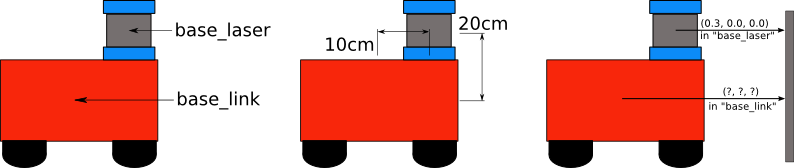
\includegraphics[width=0.5\textwidth,angle=0]{tutorials/tutorial_2/img/simple_robot.png}
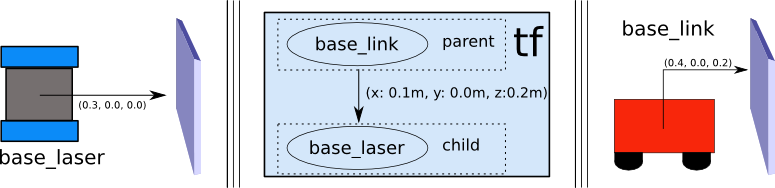
\includegraphics[width=0.5\textwidth,angle=0]{tutorials/tutorial_2/img/tf_robot.png}